\documentclass{standalone}
\usepackage{tikz}
\usepackage{amsmath}
\usepackage{bm}
\usepackage{pgfplots}
\pgfplotsset{compat=1.18}

\begin{document}

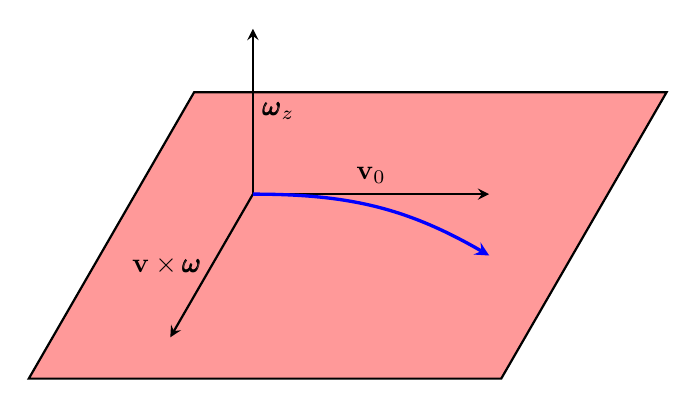
\begin{tikzpicture}[thick]
    \tikzset{arrowstyle/.style={->, >=stealth}}
    % conversion from cm to pt and vice versa
    \pgfmathsetmacro{\CmToPt}{28.3464566929}
    \pgfmathsetmacro{\PtToCm}{0.0352777778}
    

    \pgfmathsetmacro{\AxisSize}{3.0}
    \pgfmathsetmacro{\AngleAxes}{30}
    % draw the tangent plane
    \pgfmathsetmacro{\PlaneBound}{\AxisSize*1/2}     % extra boundary space around tangent plane
    \pgfmathsetmacro{\PlaneSize}{2*\PlaneBound+\AxisSize}     % extra boundary space around tangent plane
    \begin{scope}[xshift = -\PlaneBound*\CmToPt * sin(\AngleAxes), yshift= \PlaneBound * \CmToPt * cos(\AngleAxes)]
        \fill[red, opacity=0.4] (0, 0) -- (\PlaneSize, 0) -- ({\PlaneSize-sin(\AngleAxes)*\PlaneSize*0.7}, {-cos(\AngleAxes)*\PlaneSize*0.7}) -- ({-sin(\AngleAxes)*\PlaneSize*0.7}, {-cos(\AngleAxes)*\PlaneSize*0.7}) -- cycle;
        \draw (0, 0) -- (\PlaneSize, 0) -- ({\PlaneSize-sin(\AngleAxes)*\PlaneSize*0.7}, {-cos(\AngleAxes)*\PlaneSize*0.7}) -- ({-sin(\AngleAxes)*\PlaneSize*0.7}, {-cos(\AngleAxes)*\PlaneSize*0.7}) -- cycle;
    \end{scope}

    % draw the axes
    \draw[arrowstyle] (0, 0) -- (\AxisSize, 0) node[pos=0.5, above] {$\mathbf{v}_0$};
    \draw[arrowstyle] (0, 0) -- ({-sin(\AngleAxes)*\AxisSize*0.7}, {-cos(\AngleAxes)*\AxisSize*0.7}) node[pos=0.5, left] {$\mathbf{v} \times \pmb{\omega}$};
    \draw[arrowstyle] (0, 0) -- (0, \AxisSize*0.7) node[pos=0.5, right] {$\pmb{\omega}_z$};
    % draw the curved trajectory
    \draw[arrowstyle, blue, very thick] (0, 0) to[out=0, in=150] (\AxisSize, {-cos(\AngleAxes)*\AxisSize*0.3});

\end{tikzpicture}

\end{document}